\section{Performance Evaluation}
\label{sec:perf-eval}

\subsection{Evaluation criteria and reporting conventions}

Probe performance is reported with macro-F1 for the three classification tasks (voicing, real vs.\ pseudo word, orthographic transparency) and with the coefficient of determination $R^2$ for the syllable-count regression task. Reported per-model numbers are the peak across all model layers; layer-emergence figures show the full per-layer trajectory. In-language scores are computed on a held-out English split (80/20, stratified, fixed seed 42); cross-lingual scores are zero-shot transfer to the Bangla subset using the English-trained probe weights without any Bangla-side fitting. Surface-feature baselines (first-character lookup and a five-feature character-statistic baseline) are reported alongside model scores so that the \emph{gain over surface} judgement that underpins the sanity-check conclusion of Section~\ref{sec:sanity} is explicit at every step.

The chapter answers the four research questions of Section~\ref{sec:rqs} in order. Within Section~\ref{sec:perf-eval}, Section~\ref{sec:rq1} addresses RQ1 (in-language English encoding), Section~\ref{sec:sanity} reports the surface-feature sanity checks that reframe RQ1 and gate everything that follows, Section~\ref{sec:rq2} addresses RQ2 (cross-lingual transfer) on the surface-controlled subset, and Section~\ref{sec:rsa} reports Representational Similarity Analysis as a probe-free corroboration of RQ2. Section~\ref{sec:analysis} (Analysis of Design Solutions) then addresses RQ3 (mechanism and localisation) via causal forward-hook ablation and extends it to a depth-and-overlap analysis on mT5. Section~\ref{sec:adjustments} reports the design adjustments made as a direct consequence of these results, Section~\ref{sec:stats} reports the statistical-analysis conventions, Section~\ref{sec:comparisons} addresses RQ4 (cross-model comparison and model selection) and the relationship to prior work, and Section~\ref{sec:discussion} interprets the joint pattern.

The headline results of the chapter are summarised across the three figures that follow. Figure~\ref{fig:summary-sanity} establishes the surface-feature sanity checks and the length-matched recovery; Figure~\ref{fig:summary-transfer} reports zero-shot cross-lingual transfer and causal-ablation specificity; Figure~\ref{fig:summary-mt5} reports the mT5 localisation analysis. All four model families share the same frozen-LLM pipeline and the same 440-stimulus dataset.

\begin{figure}[H]
\centering
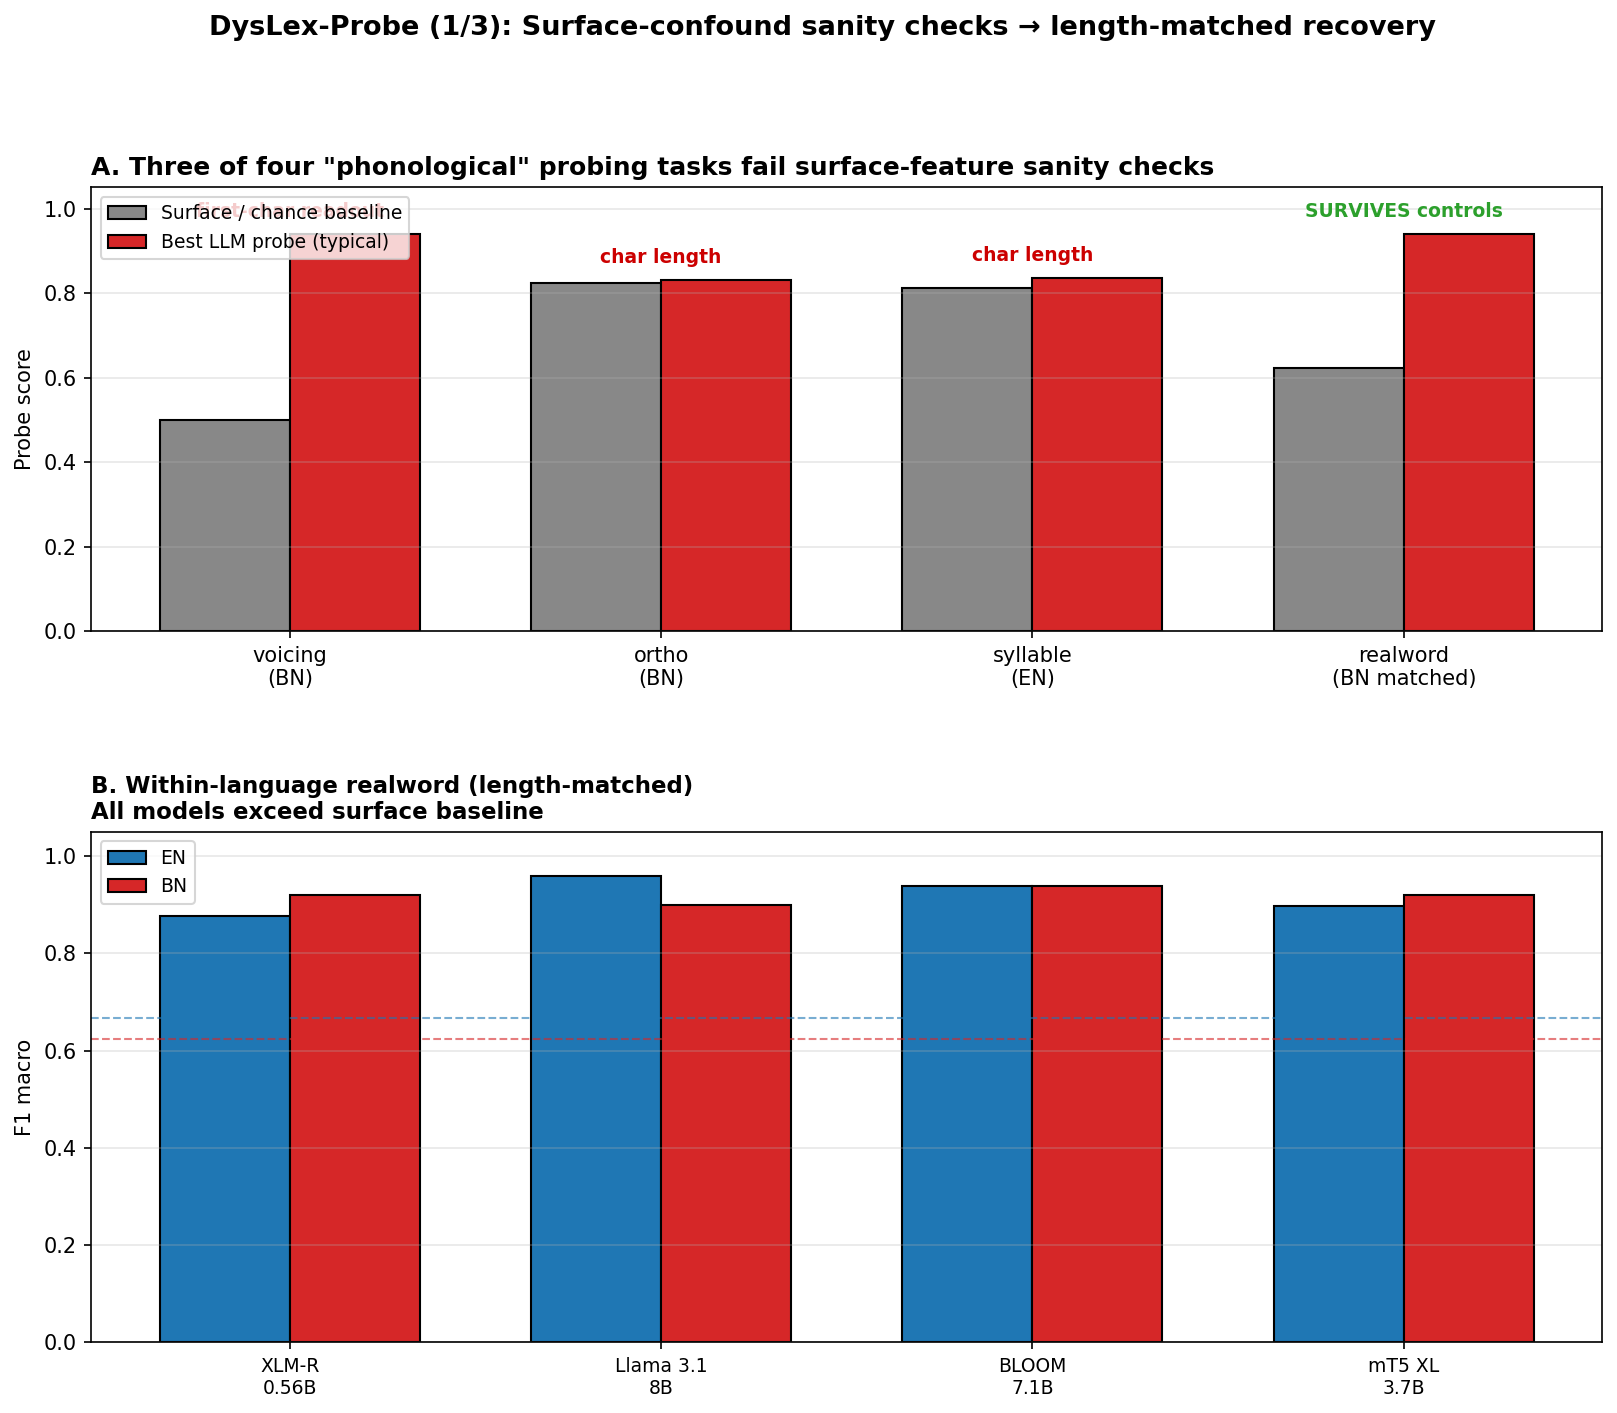
\includegraphics[width=0.95\textwidth]{plots_summary_1_sanity_realword.png}
\caption{Surface-confound sanity checks and length-matched recovery. (A) Three of four ``phonological'' probing tasks fail surface-feature sanity checks; only length-matched real-versus-pseudo word survives. (B) On the length-matched real-word subset, every model exceeds its within-language surface baseline in both English and Bangla.}
\label{fig:summary-sanity}
\end{figure}

\begin{figure}[H]
\centering
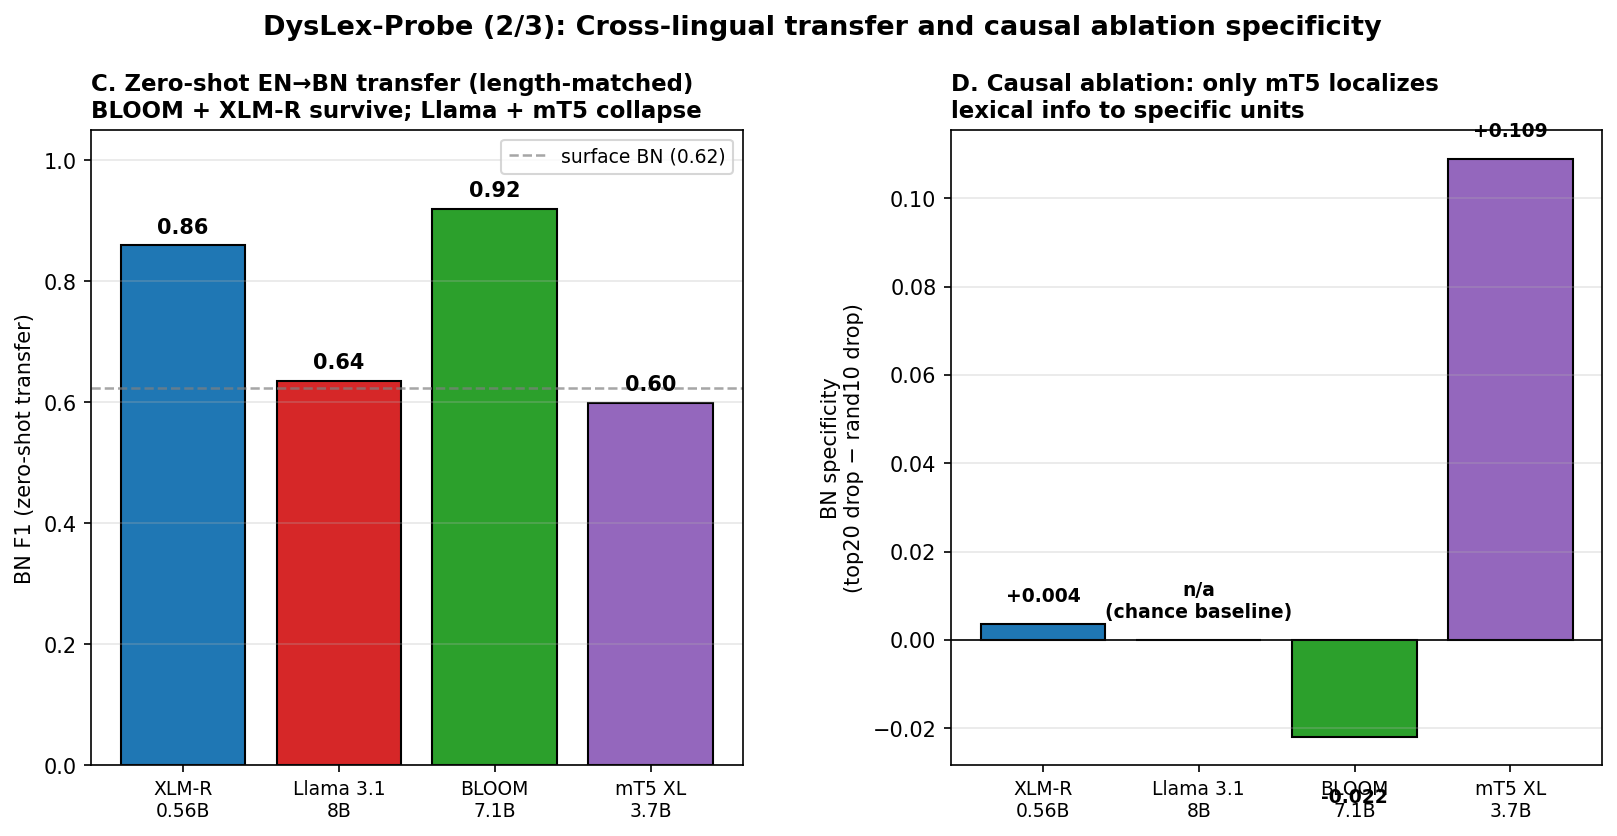
\includegraphics[width=0.95\textwidth]{plots_summary_2_transfer_ablation.png}
\caption{Cross-lingual transfer and causal ablation. (C) Zero-shot English$\rightarrow$Bangla transfer on the length-matched subset: BLOOM and XLM-R survive above the surface baseline, while Llama and mT5 collapse to it. (D) Causal ablation specificity (top-20 drop minus random-10 drop): only mT5 localises lexical information to specific units; Llama is undefined as its baseline sits at chance.}
\label{fig:summary-transfer}
\end{figure}

\begin{figure}[H]
\centering
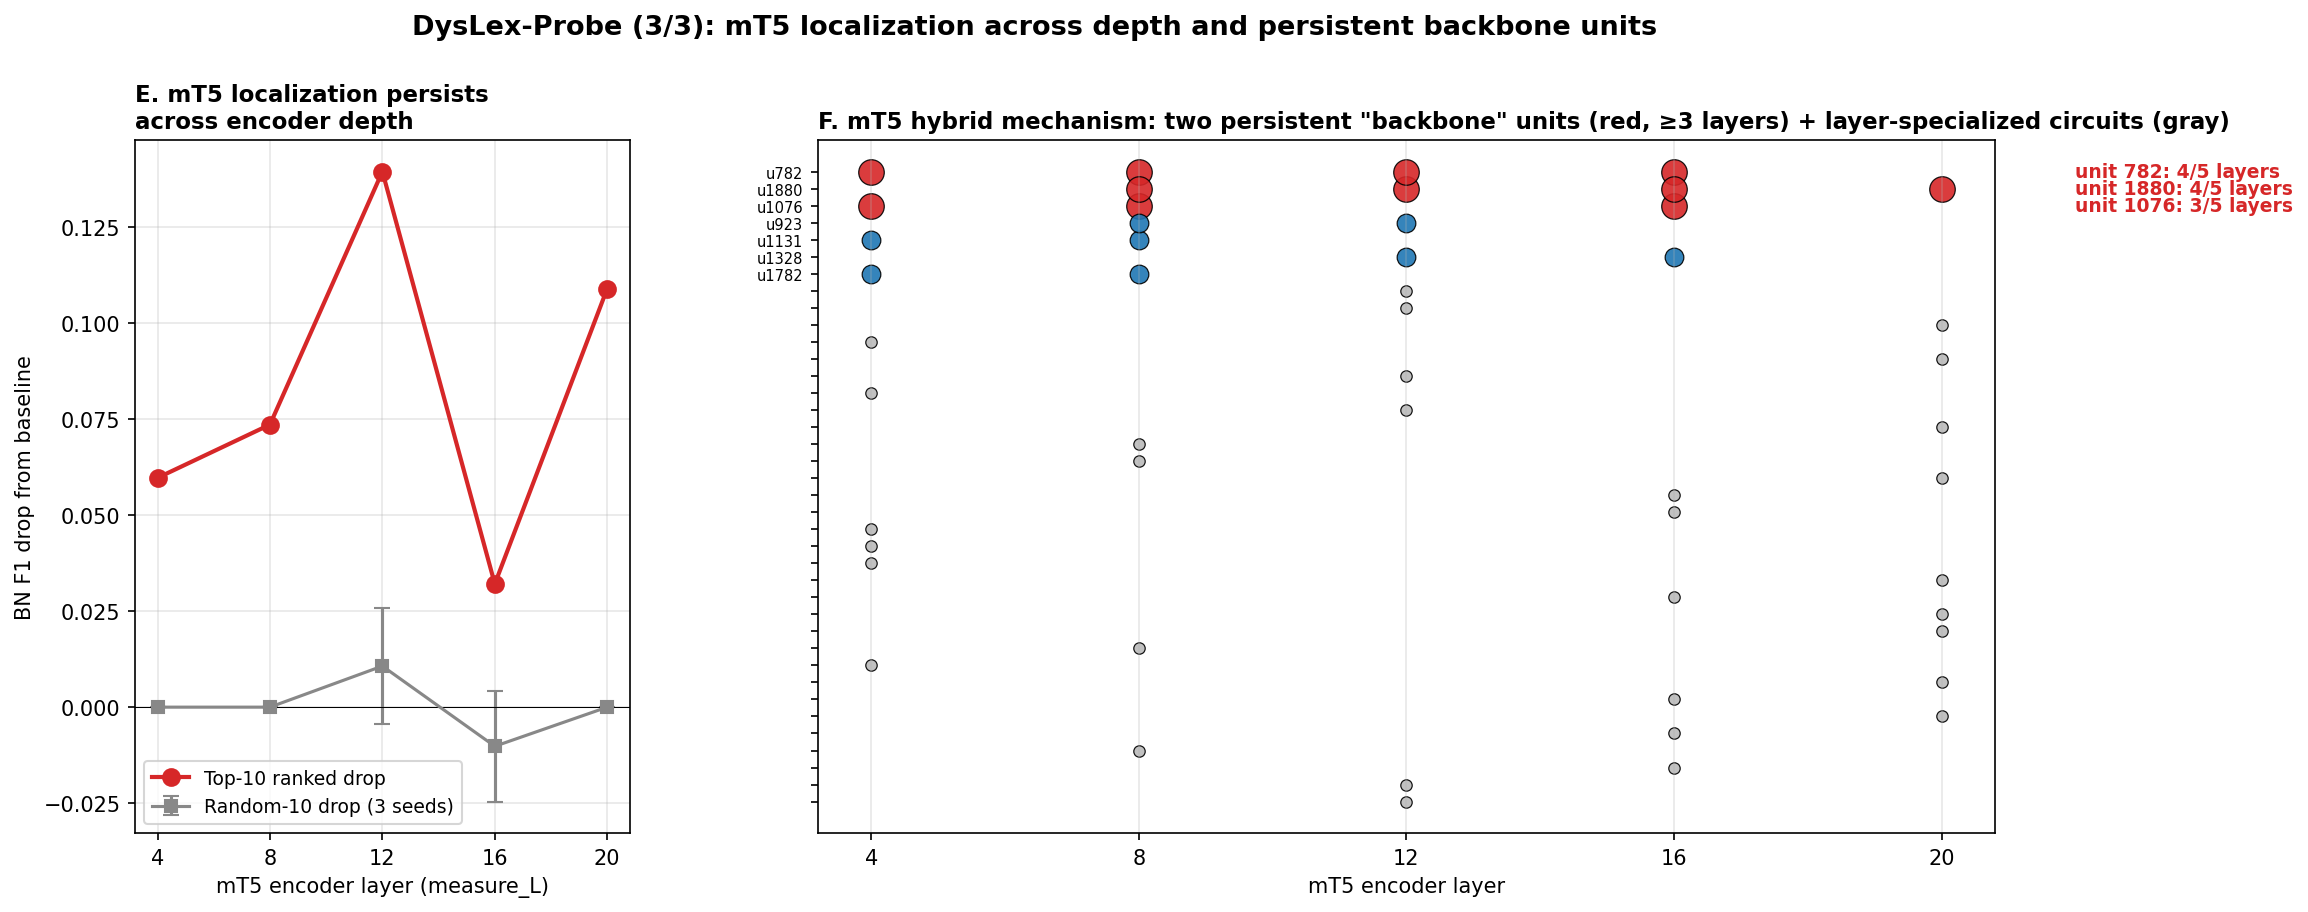
\includegraphics[width=\textwidth]{plots_summary_3_mt5_localization.png}
\caption{mT5 localisation mechanism. (E) The ranked-unit ablation drop exceeds the random-unit drop across encoder depth, so localisation persists rather than being a single-layer artefact. (F) Two persistent ``backbone'' units (red, present in $\geq 3$ of five probed layers) coexist with layer-specialised circuits (gray), indicating a hybrid distributed-plus-localised mechanism.}
\label{fig:summary-mt5}
\end{figure}

\subsection{RQ1: In-language English probing across the four models}
\label{sec:rq1}

Table~\ref{tab:rq1-en} reports per-model peak in-language English performance on the four phonological probing tasks; Figure~\ref{fig:four-english} visualises the per-layer trajectories.

\begin{table}[H]
\centering
\caption{In-language English probing (RQ1): peak layer / peak score per model per task. F1 for voicing, realword, ortho; $R^{2}$ for syllable.}
\label{tab:rq1-en}
\small
\resizebox{\textwidth}{!}{%
\setlength{\tabcolsep}{10pt}
\renewcommand{\arraystretch}{2}
\begin{tabular}{|c|c|c|c|c|}
\hline
\textbf{Task} & \textbf{XLM-R} & \textbf{Llama} & \textbf{BLOOM} & \textbf{mT5} \\
\hline
voicing  & L11 / 0.62 & L2  / 0.73 & L6  / 0.55 & L9  / 0.58 \\
\hline
realword & L11 / 0.84 & L12 / 0.91 & L22 / 0.79 & L24 / 0.81 \\
\hline
ortho    & L0  / 0.92 & L32 / 0.71 & L12 / 0.68 & L21 / 0.69 \\
\hline
syllable & L8  / 0.67 & L16 / 0.70 & L29 / 0.68 & L20 / 0.76 \\
\hline
\end{tabular}%
}
\end{table}

\begin{figure}[H]
\centering
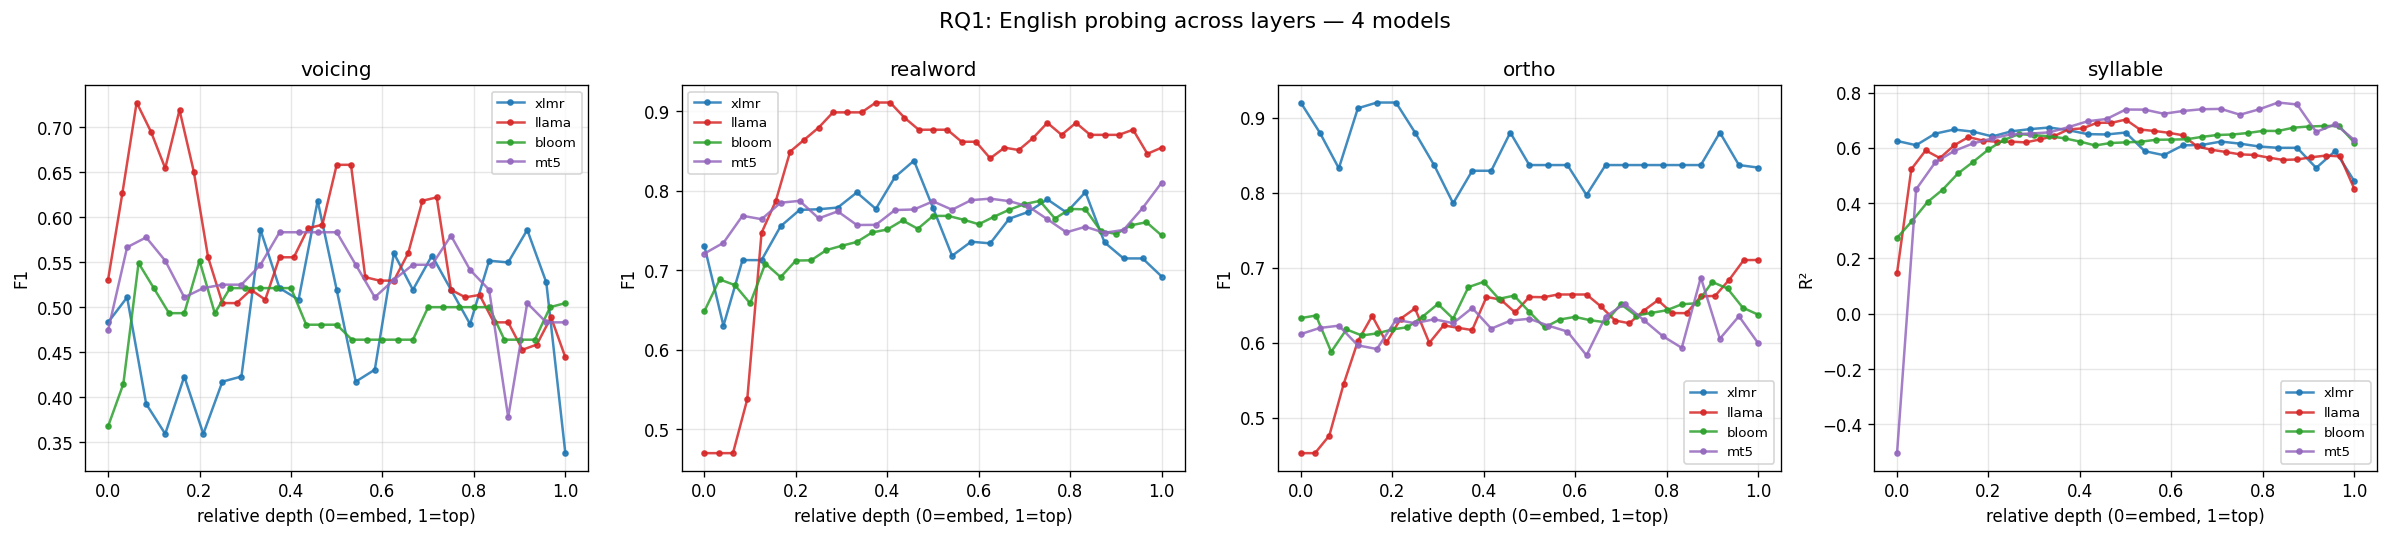
\includegraphics[width=0.95\textwidth]{plots_four_models_english.png}
\caption{Per-layer in-language English probing performance across the four models on voicing, realword, orthographic transparency and syllable count.}
\label{fig:four-english}
\end{figure}

\textbf{Layer-emergence patterns.} The layer-emergence trajectories (Figure~\ref{fig:layer-emergence}) differ across architectures in ways that are interpretable in the light of each model's pretraining objective. XLM-R, the multilingual masked encoder, peaks for the realword task in its middle layers (L11), consistent with prior probing findings that masked encoders concentrate lexical and morphological structure in mid-network and reserve final layers for task-conditional reorganisation \cite{hewitt2019structural,belinkov2022probing}. Llama, the English-causal decoder, peaks early for voicing (L2) and late for syllable count (L16); early-layer voicing signal is consistent with the first-character recovery pattern surfaced in Section~\ref{sec:sanity}, while later-layer syllable count requires the integration of multi-token spans that only emerges as causal attention has had enough depth to aggregate. BLOOM, also a causal decoder but trained on 46 languages, peaks late for realword (L22), suggesting that multilingual subword combinatorics in a causal decoder accrue toward the top of the stack. mT5's encoder peaks at the top of its 24-layer encoder for realword (L24) and slightly earlier for syllable and ortho (L20--L21); span-corruption pretraining appears to push lexical-like content toward the top of the encoder where the decoder will read it.

These early-middle-late patterns are suggestive but cannot be read at face value: before they are interpreted as architectural facts about phonological encoding, the apparent scores in Table~\ref{tab:rq1-en} must survive surface-feature sanity checks (Section~\ref{sec:sanity}). Three of the four tasks do not survive.

\begin{figure}[H]
\centering
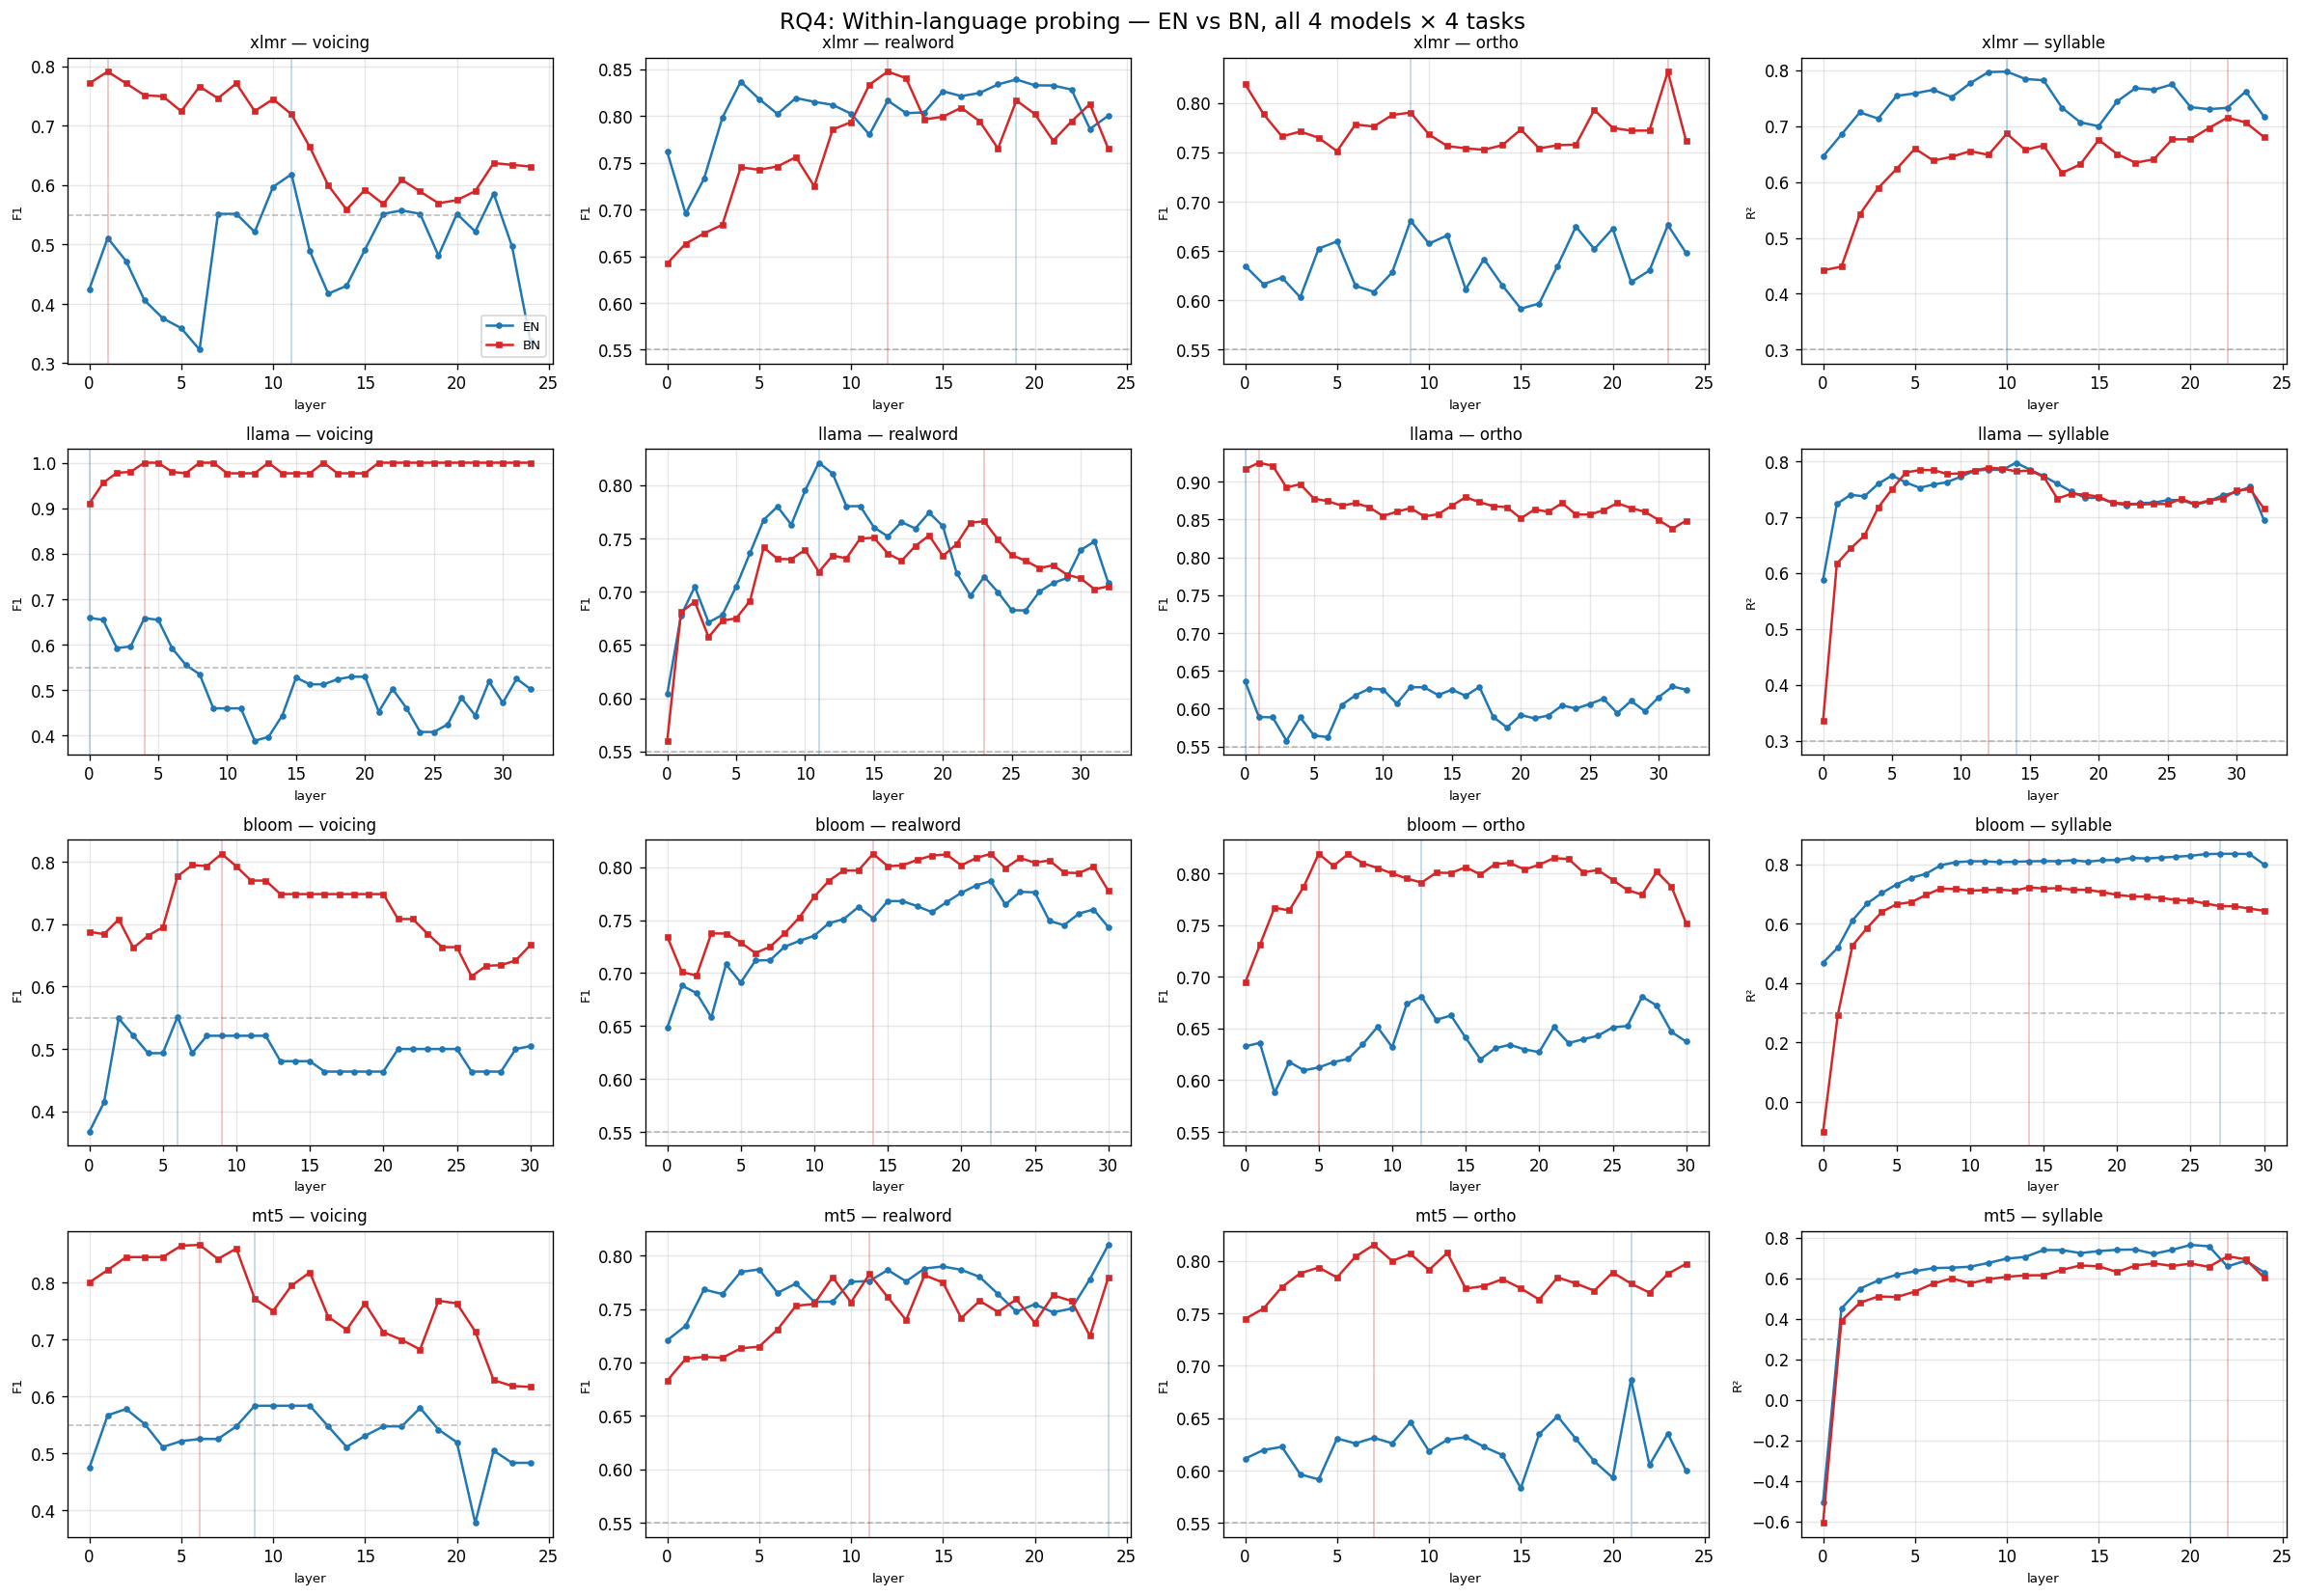
\includegraphics[width=0.95\textwidth]{plots_layer_emergence_all_models.png}
\caption{Layer-emergence trajectories across all four models on the four probing tasks. Subplots align across rows by task; the layer axis is normalised to relative encoder depth.}
\label{fig:layer-emergence}
\end{figure}

\subsection{Surface-feature sanity checks invalidate three of four tasks}
\label{sec:sanity}

The apparent scores in Table~\ref{tab:rq1-en} are striking. Before they are read as phonological evidence, three sanity-check baselines are applied (full methodology in Chapter~4 \S{Surface-feature sanity checks}). The first reads the voicing label off the first character of the word; the second tests whether a five-feature character-statistic baseline beats the LLM probes on orthographic transparency and syllable count; the third matches real and pseudo words on character length within each language and re-probes.

\subsubsection{Voicing: Bangla labels are recoverable from the first character alone}

A leave-one-out probe trained on the layer-0 token-embedding state with a one-hot encoding of the first character recovers Bangla voicing labels with F1 between 0.78 and 0.94 across the four models (Table~\ref{tab:sanity-voicing}); the deterministic upper bound, a rule that reads the first character and assigns voicing, is 1.00. In other words, 100\% of Bangla voicing labels in the stimulus set are inferable from the first character. The probe is therefore reading token identity, not phonological voicing. All Bangla voicing numbers reported in Table~\ref{tab:rq1-en} for RQ1, and any cross-lingual or causal-ablation number subsequently derived from them, reflect first-character recognition rather than a phonological feature.

\begin{table}[H]
\centering
\caption{First-character lookup sanity check (Bangla voicing). LOO F1 at layer~0 versus peak across layers, and deterministic upper bound. All numbers indicate that the voicing label is encoded by the first character of the word.}
\label{tab:sanity-voicing}
\small
\resizebox{\textwidth}{!}{%
\setlength{\tabcolsep}{10pt}
\renewcommand{\arraystretch}{2}
\begin{tabular}{|c|c|c|c|}
\hline
\textbf{Model} & \textbf{L0 LOO F1} & \textbf{Peak LOO F1} & \textbf{Deterministic upper bound} \\
\hline
XLM-R  & 0.80 & 0.83          & 1.00 \\
\hline
Llama  & 0.94 & 1.00 (L2+)    & 1.00 \\
\hline
BLOOM  & 0.78 & 0.80          & 1.00 \\
\hline
mT5    & 0.80 & 0.87          & 1.00 \\
\hline
\end{tabular}%
}
\end{table}

\begin{figure}[H]
\centering
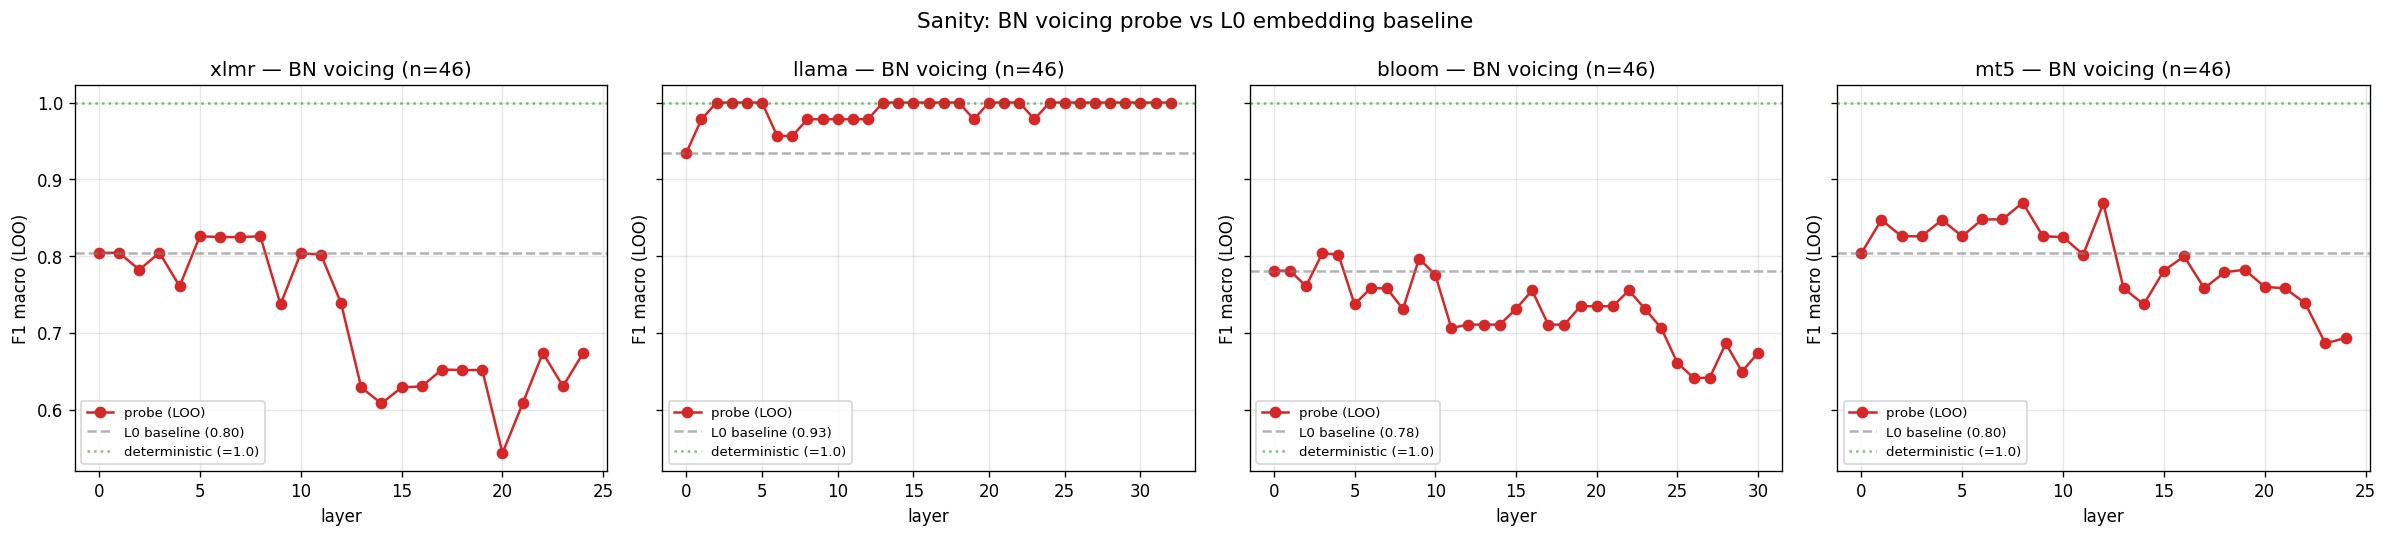
\includegraphics[width=0.85\textwidth]{plots_bn_voicing_sanity.png}
\caption{Bangla voicing sanity check: per-layer leave-one-out probe trained on layer-0 token embeddings recovers voicing labels at F1 0.78--0.94, indicating the labels are inferable from first-character identity alone. The probe is not reading phonological voicing.}
\label{fig:bn-voicing-sanity}
\end{figure}

\subsubsection{Orthographic transparency: solved by character length}

A five-feature surface baseline (character length, byte length, unique-character count, vowel ratio, longest consonant run) reaches F1 0.66 in English and 0.82 in Bangla on the orthographic-transparency task. The best LLM probes gain $\leq +0.03$ in English and $\leq +0.01$ in Bangla over this baseline. The LLM representations do not contribute information above a five-feature character-statistic baseline on this task; the orthographic-transparency task as posed in the stimulus set is a surface task.

\subsubsection{Syllable count: surface-confounded}

The same five-feature baseline reaches $R^2 = 0.81$ on English syllable count and $R^2 = 0.67$ on Bangla. Three of the four LLMs (Llama, mT5, XLM-R) \emph{under-perform} the surface baseline in English; only BLOOM gains $+0.02$. The syllable-count task is also surface-driven.

\subsubsection{Real vs.\ pseudo word: survives length matching}

When real and pseudo words are matched 1:1 on character length (50 matched per language; mean character length 6.88 in English, 5.20 in Bangla), all four models gain at least $+0.20$ F1 over both their layer-0 and the five-feature surface baseline on Bangla (Table~\ref{tab:realword-matched}). The real-versus-pseudo word task is the only one of the four that passes the surface-feature controls and is the only task on which the remainder of this chapter reports cross-lingual transfer, RSA and causal-ablation numbers.

\begin{table}[H]
\centering
\caption{Length-matched realword probing per language. EN/BN at layer 0 versus peak layer, with gain over L0. All four models gain $\geq +0.20$ F1 on Bangla; this is the only task that passes surface-feature controls.}
\label{tab:realword-matched}
\small
\resizebox{\textwidth}{!}{%
\setlength{\tabcolsep}{10pt}
\renewcommand{\arraystretch}{2}
\begin{tabular}{|c|c|c|c|c|c|c|}
\hline
\textbf{Model} & \textbf{EN L0} & \textbf{EN peak} & \textbf{EN gain} & \textbf{BN L0} & \textbf{BN peak} & \textbf{BN gain} \\
\hline
XLM-R & 0.81 & 0.88 & +0.06 & 0.66 & \textbf{0.92} & \textbf{+0.25} \\
\hline
Llama & 0.75 & 0.96 & +0.21 & 0.64 & \textbf{0.90} & \textbf{+0.26} \\
\hline
BLOOM & 0.81 & 0.94 & +0.13 & 0.64 & \textbf{0.94} & \textbf{+0.30} \\
\hline
mT5   & 0.65 & 0.90 & +0.23 & 0.72 & \textbf{0.92} & \textbf{+0.20} \\
\hline
\end{tabular}%
}
\end{table}

\subsection{RQ2: Length-matched cross-lingual transfer}
\label{sec:rq2}

The English-trained length-matched realword probe is evaluated zero-shot on the Bangla length-matched subset. Table~\ref{tab:transfer-matched} reports the surface-controlled cross-lingual numbers; Figures~\ref{fig:four-transfer} and \ref{fig:transfer-matched} visualise the per-layer trajectories and the headline surface-controlled comparison respectively.

\begin{table}[H]
\centering
\caption{Length-matched cross-lingual transfer (EN $\rightarrow$ BN). Peak layer / peak BN F1 / gain over surface baseline / verdict. After surface controls only XLM-R and BLOOM transfer; Llama and mT5 collapse.}
\label{tab:transfer-matched}
\small
\resizebox{\textwidth}{!}{%
\setlength{\tabcolsep}{10pt}
\renewcommand{\arraystretch}{2}
\begin{tabular}{|c|c|c|c|c|}
\hline
\textbf{Model} & \textbf{Peak L (rel.)} & \textbf{Peak BN F1} & \textbf{Gain over surface} & \textbf{Verdict} \\
\hline
XLM-R & L16 / rel.\ 0.67 & \textbf{0.86} & \textbf{+0.24} & real transfer \\
\hline
BLOOM & L25 / rel.\ 0.83 & \textbf{0.92} & \textbf{+0.30} & real transfer \\
\hline
Llama & L31 / rel.\ 0.97 & 0.63          & +0.01           & collapsed to surface \\
\hline
mT5   & L20 / rel.\ 0.83 & 0.60          & $-0.02$         & collapsed below surface \\
\hline
\end{tabular}%
}
\end{table}

The negative entry for mT5 ($-0.02$) does not indicate anti-learning. It means the length-matched Bangla probe built on mT5 representations scores marginally \emph{below} the five-feature character-statistic surface baseline: the representation carries no cross-lingual real-versus-pseudo word information beyond surface statistics, and the small negative magnitude is within the estimation noise of the $n = 50$ matched subset. Operationally it is read as zero transfer, the same interpretation as Llama's $+0.01$; the sign is not meaningful, only the absence of a positive gain over surface.

\begin{figure}[H]
\centering
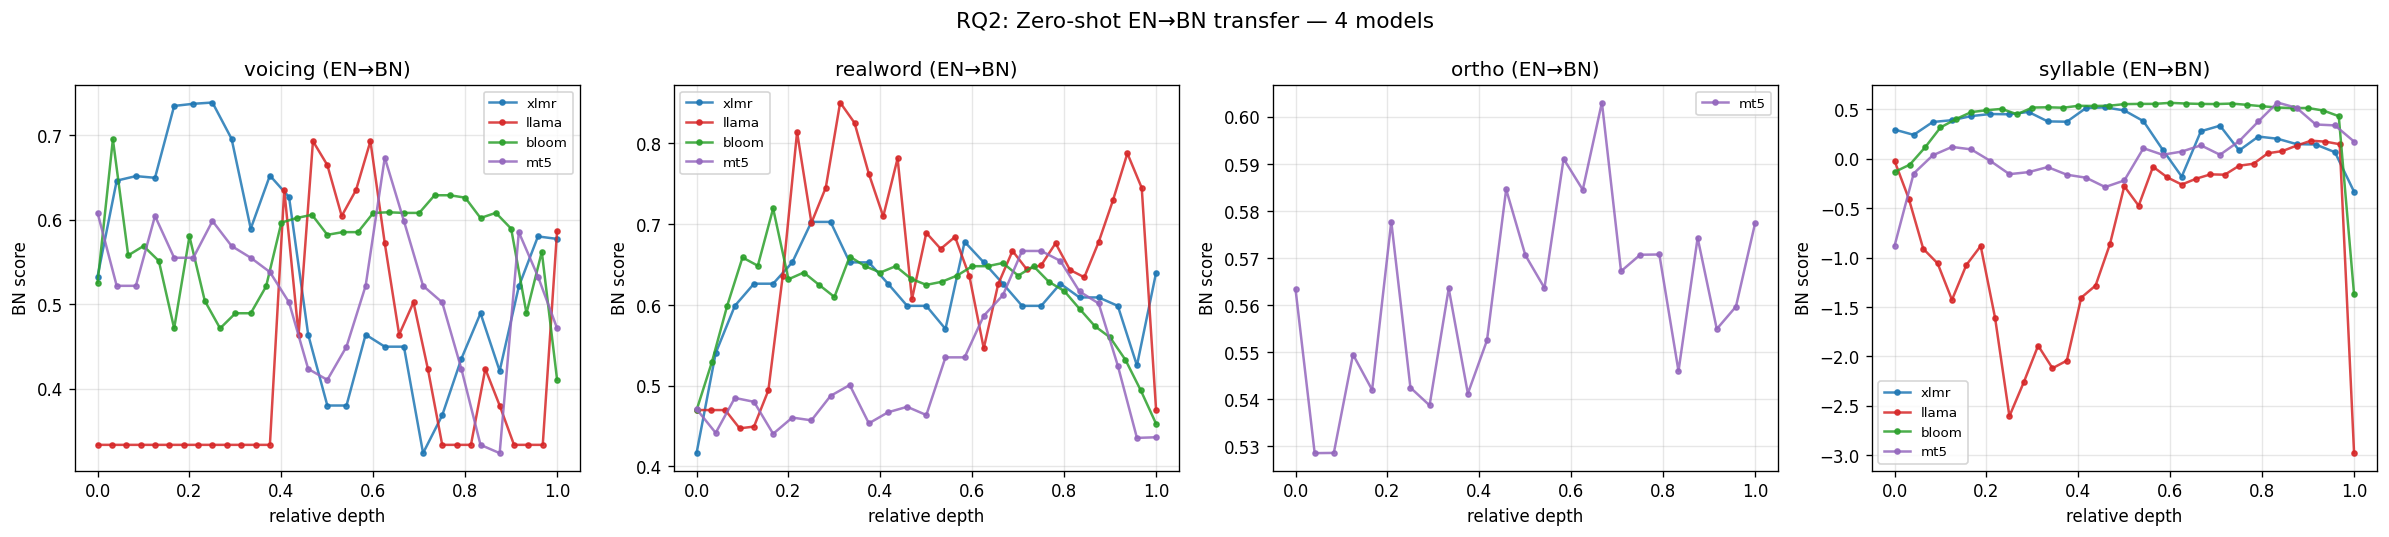
\includegraphics[width=0.95\textwidth]{plots_four_models_transfer.png}
\caption{Per-layer cross-lingual transfer (EN $\rightarrow$ BN) across the four models on all four tasks. Voicing, ortho and syllable curves reflect surface confounds (Section~\ref{sec:sanity}); only the realword curve, length-matched, is interpretable.}
\label{fig:four-transfer}
\end{figure}

\begin{figure}[H]
\centering
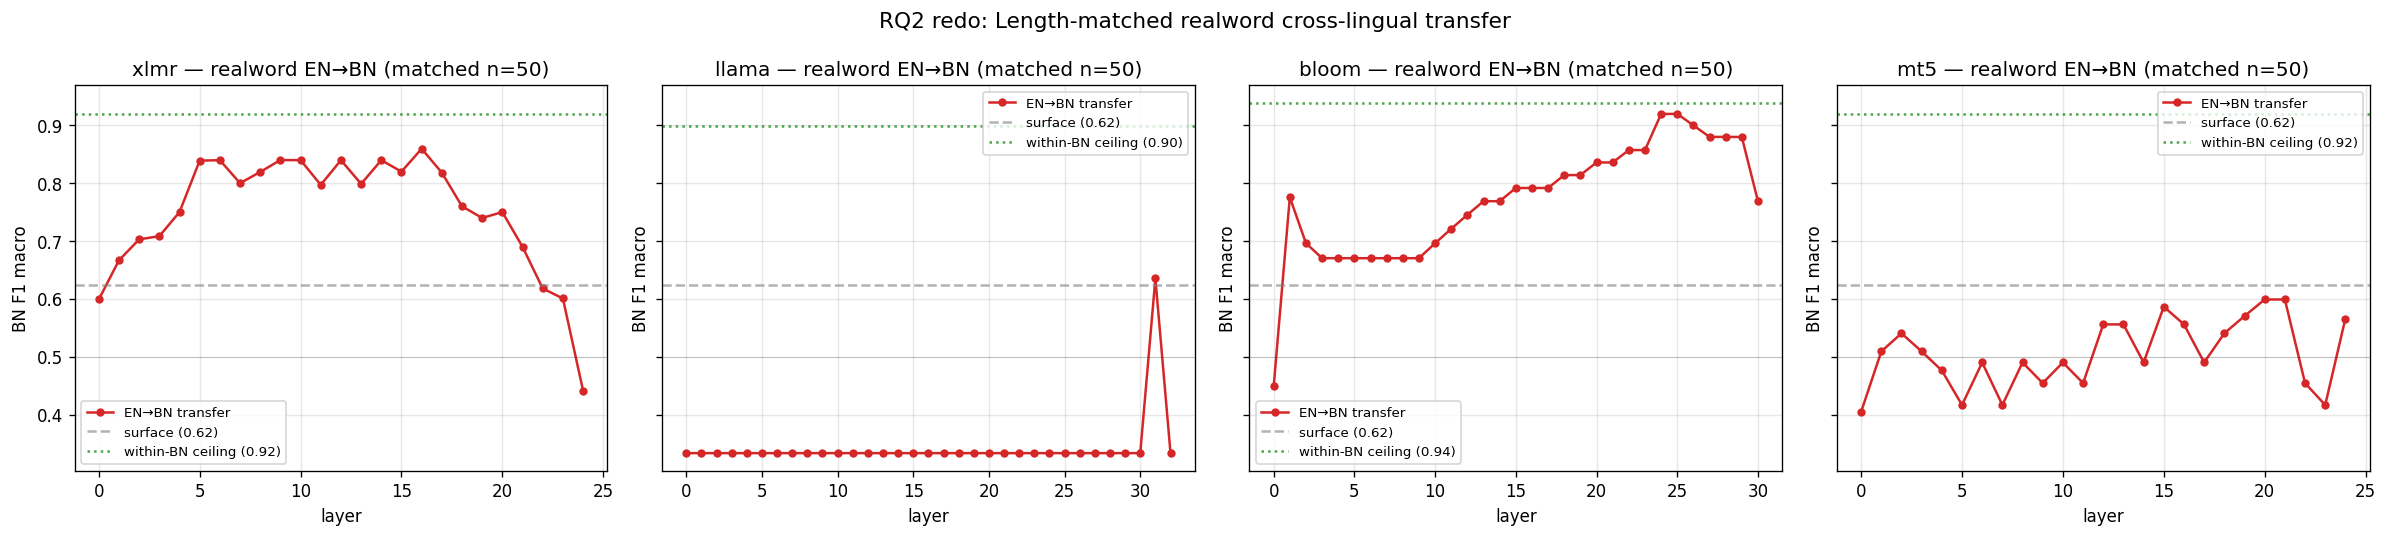
\includegraphics[width=0.95\textwidth]{plots_transfer_realword_matched.png}
\caption{Surface-controlled length-matched real vs.\ pseudo word cross-lingual transfer. XLM-R and BLOOM achieve genuine transfer ($+0.24$ and $+0.30$ over surface respectively); Llama and mT5 collapse to surface level.}
\label{fig:transfer-matched}
\end{figure}

After surface controls only the multilingual masked encoder (XLM-R) and the multilingual causal decoder (BLOOM) achieve genuine cross-lingual real-versus-pseudo word transfer; the English-causal decoder (Llama) and the multilingual span-corruption encoder-decoder (mT5) collapse to surface-baseline level. Two implications follow.

First, pretraining objective and language coverage \emph{jointly} determine cross-lingual transfer. BLOOM beats Llama at similar parameter scale because BLOOM has explicit Bangla coverage in its pretraining mix; XLM-R beats Llama at roughly $13\times$ smaller parameter count because XLM-R is a multilingual MLM encoder. Architecture family alone (encoder-only vs.\ decoder-only) is not predictive: both XLM-R and BLOOM transfer, with very different architectures. Coverage alone (multilingual vs.\ English-heavy) is also not sufficient: mT5 is multilingual and yet collapses; its span-corruption objective appears not to surface cross-lingual lexical similarity at the probe-readable level.

Second, in-language English performance is not a reliable predictor of cross-lingual transfer. Llama reaches the highest in-language English realword F1 (0.96) and the lowest cross-lingual Bangla F1 (0.63); the gap is fully explained by pretraining language coverage. Selecting a model substrate for low-resource Bangla on the basis of English benchmark numbers alone would have picked the worst-transferring model in this comparison.

\subsection{Representational Similarity Analysis corroborates the transfer split}
\label{sec:rsa}

Probing measures whether a feature is linearly recoverable from a representation; Representational Similarity Analysis (RSA) tests whether the geometry of stimulus representations is preserved across languages, independent of any downstream probe. The two methods give consistent answers.

Cross-lingual Representational Dissimilarity Matrix (RDM) Spearman $\rho$ and English $\rightarrow$ Bangla mate-retrieval Top-1 accuracy peak at mid layers for the two transferring models. XLM-R reaches its highest cross-lingual RDM correlation in its middle encoder layers (Figure~\ref{fig:rsa-xlmr}), coincident with the layer at which the length-matched realword probe transfers (L16 in Table~\ref{tab:transfer-matched}). BLOOM reaches Top-1 $0.65$ at L4. Llama reaches Top-1 $0.85$ at L6 in the \emph{unmatched} RSA setting, but this is driven by the same surface confound that inflates its unmatched probing numbers and is reframed by the length-matched probe collapse (Table~\ref{tab:transfer-matched}). The RSA result therefore corroborates the surface-controlled probing result: representational geometry is preserved cross-lingually in XLM-R and BLOOM but not in mT5.

\begin{figure}[H]
\centering
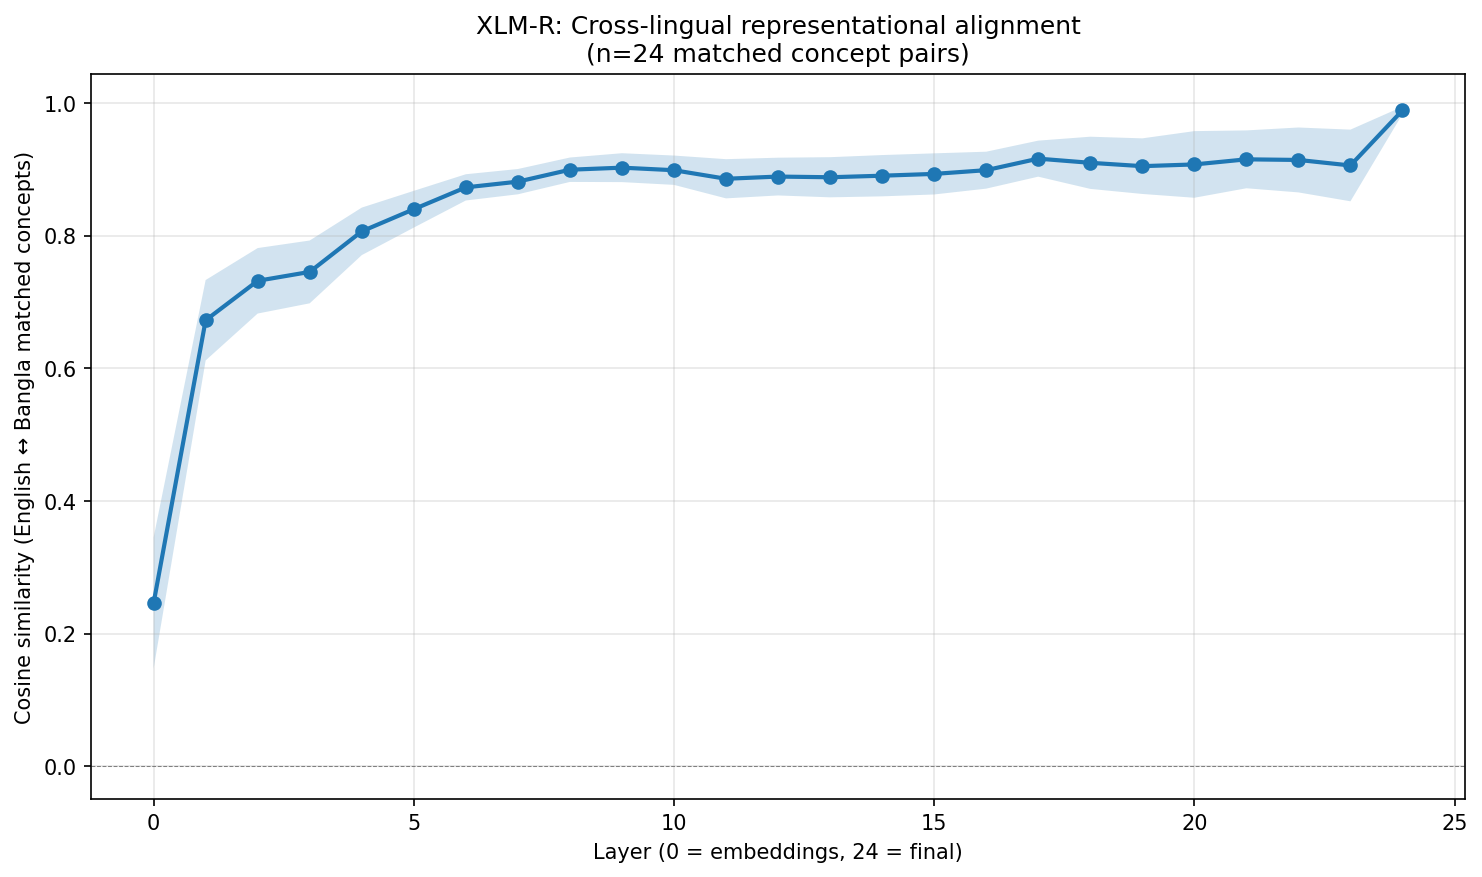
\includegraphics[width=0.75\textwidth]{plots_rsa.png}
\caption{Representational Similarity Analysis for XLM-R: cross-lingual RDM Spearman $\rho$ per layer, with the mate-retrieval Top-1 trajectory overlaid. The mid-encoder peak coincides with the layer at which the length-matched realword probe transfers.}
\label{fig:rsa-xlmr}
\end{figure}

\section{Analysis of Design Solutions}
\label{sec:analysis}

This section addresses RQ3 (mechanism and localisation) by causally testing where each model's cross-lingual lexical signal lives. The analysis combines forward-hook ablation on all four models (Section~\ref{sec:rq3}) with a depth-and-overlap extension on the mT5 encoder (Section~\ref{sec:mt5-localisation}).

\subsection{RQ3: Causal forward-hook ablation on length-matched realword}
\label{sec:rq3}

For each model the length-matched realword probe is first trained on English at the chosen \texttt{measure\_L} layer; ablation hooks three layers earlier zero either the top-20 probe-ranked units or a random-20 control set (averaged over three seeds), and the drop in Bangla F1 is measured. \emph{Ablation specificity} (the top-$K$ drop minus the random-$K$ drop, defined in Chapter~4) is positive when the probe-ranked units carry the causally relevant information, near zero for a distributed encoding, and negative when redundancy is partially undone by ablation.

\begin{table}[H]
\centering
\caption{Causal forward-hook ablation on length-matched realword. mT5 alone shows selective localisation; XLM-R and BLOOM distribute lexical information; Llama has no BN transfer to disrupt.}
\label{tab:ablation-four}
\small
\resizebox{\textwidth}{!}{%
\setlength{\tabcolsep}{10pt}
\renewcommand{\arraystretch}{2}
\begin{tabular}{|c|c|c|c|c|c|}
\hline
\textbf{Model} & \textbf{measure\_L} & \textbf{BN baseline} & \textbf{top20 drop} & \textbf{rand10 drop} & \textbf{specificity} \\
\hline
XLM-R & L8  & 0.78 & $+0.03$    & $+0.02$    & $+0.004$ \\
\hline
Llama & L11 & 0.33 & $0.000$    & $0.000$    & n/a (BN = chance) \\
\hline
BLOOM & L19 & 0.81 & $-0.02$    & $0.00$     & $-0.02$ \\
\hline
\textbf{mT5} & \textbf{L20} & \textbf{0.60} & $\bm{+0.11}$ & \textbf{0.00} & $\bm{+0.11}$ \\
\hline
\end{tabular}%
}
\end{table}

Four observations follow from Table~\ref{tab:ablation-four}.

\textbf{mT5 shows clean specificity.} Zeroing the top-20 probe-ranked units at L17 (three layers below the L20 measure point) drops the Bangla F1 by 0.11, while a random-20 control causes no drop at all. The cross-lingual lexical signal in mT5 is therefore concentrated, not distributed.

\textbf{XLM-R distributes the signal.} Top-20 and random-20 ablation produce essentially the same drop ($+0.03$ vs.\ $+0.02$), so specificity is $+0.004$ (within seed noise). The cross-lingual lexical signal is widely distributed across XLM-R's hidden units; no small subset is causally privileged.

\textbf{BLOOM is also distributed, with mild redundancy.} Specificity is marginally negative ($-0.02$): zeroing the top-20 probe-ranked units slightly \emph{improves} Bangla transfer. This is consistent with distributed redundancy, where multiple unit groups carry overlapping copies of the signal and zeroing one group lets the others dominate. The finding is reported honestly rather than masked.

\textbf{Llama has no BN transfer to disrupt.} Llama's length-matched Bangla baseline is at chance (0.33 F1 with chance $\approx 0.50$ for two-class macro F1; the model's English-trained probe assigns essentially no useful weight to Bangla representations), so ablation can neither improve nor degrade transfer and specificity is not defined.

\begin{figure}[H]
\centering
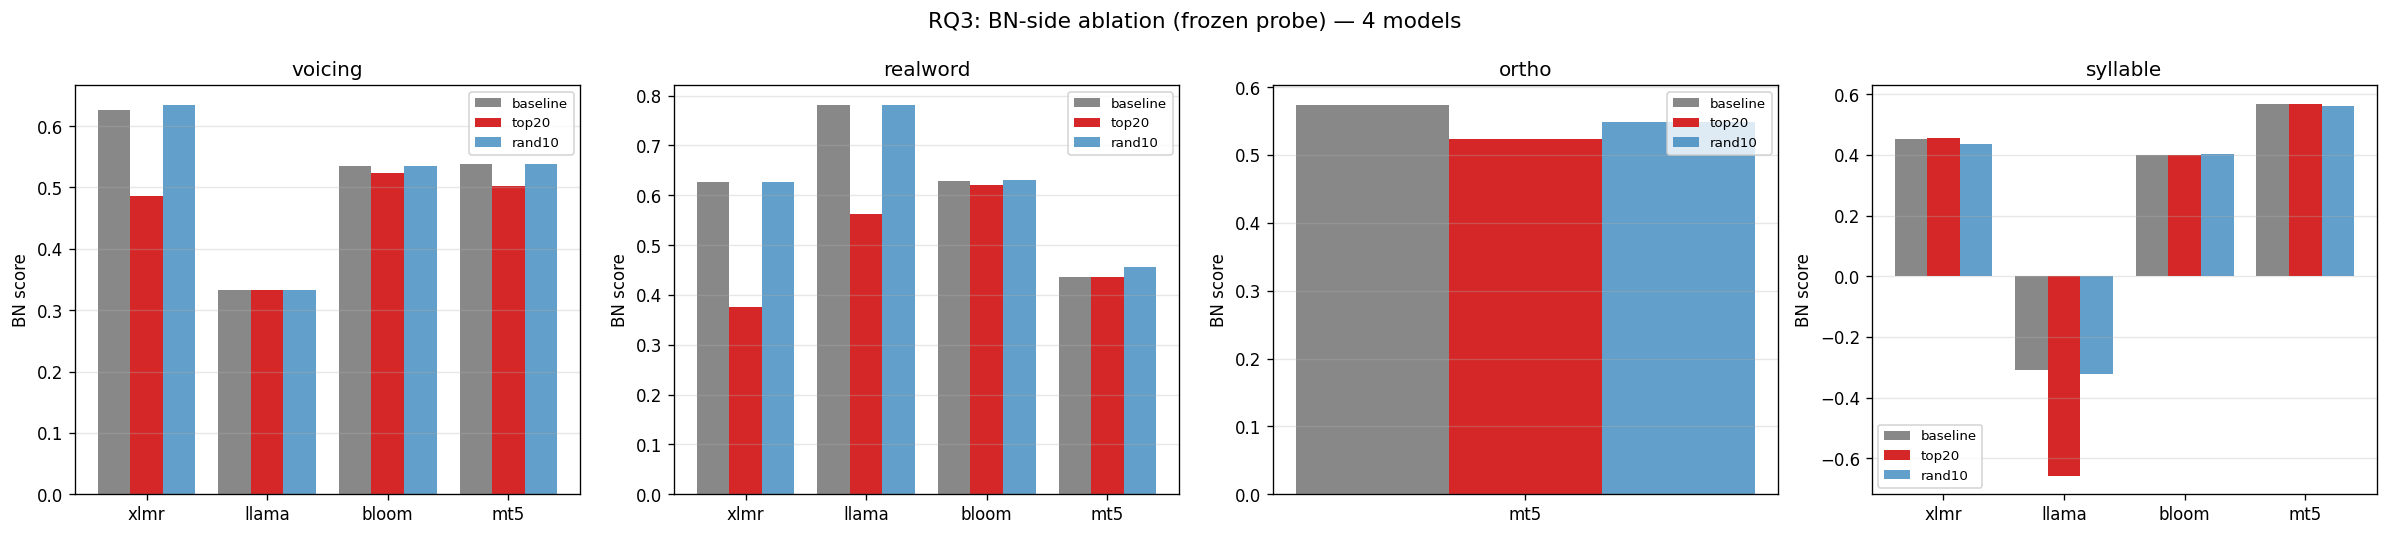
\includegraphics[width=0.95\textwidth]{plots_four_models_ablation.png}
\caption{Four-model causal ablation on length-matched realword. Top-$K$ versus random-$K$ unit ablation on Bangla cross-lingual probe. mT5 shows clean specificity ($+0.11$); XLM-R, BLOOM and Llama do not.}
\label{fig:four-ablation}
\end{figure}

\begin{figure}[H]
\centering
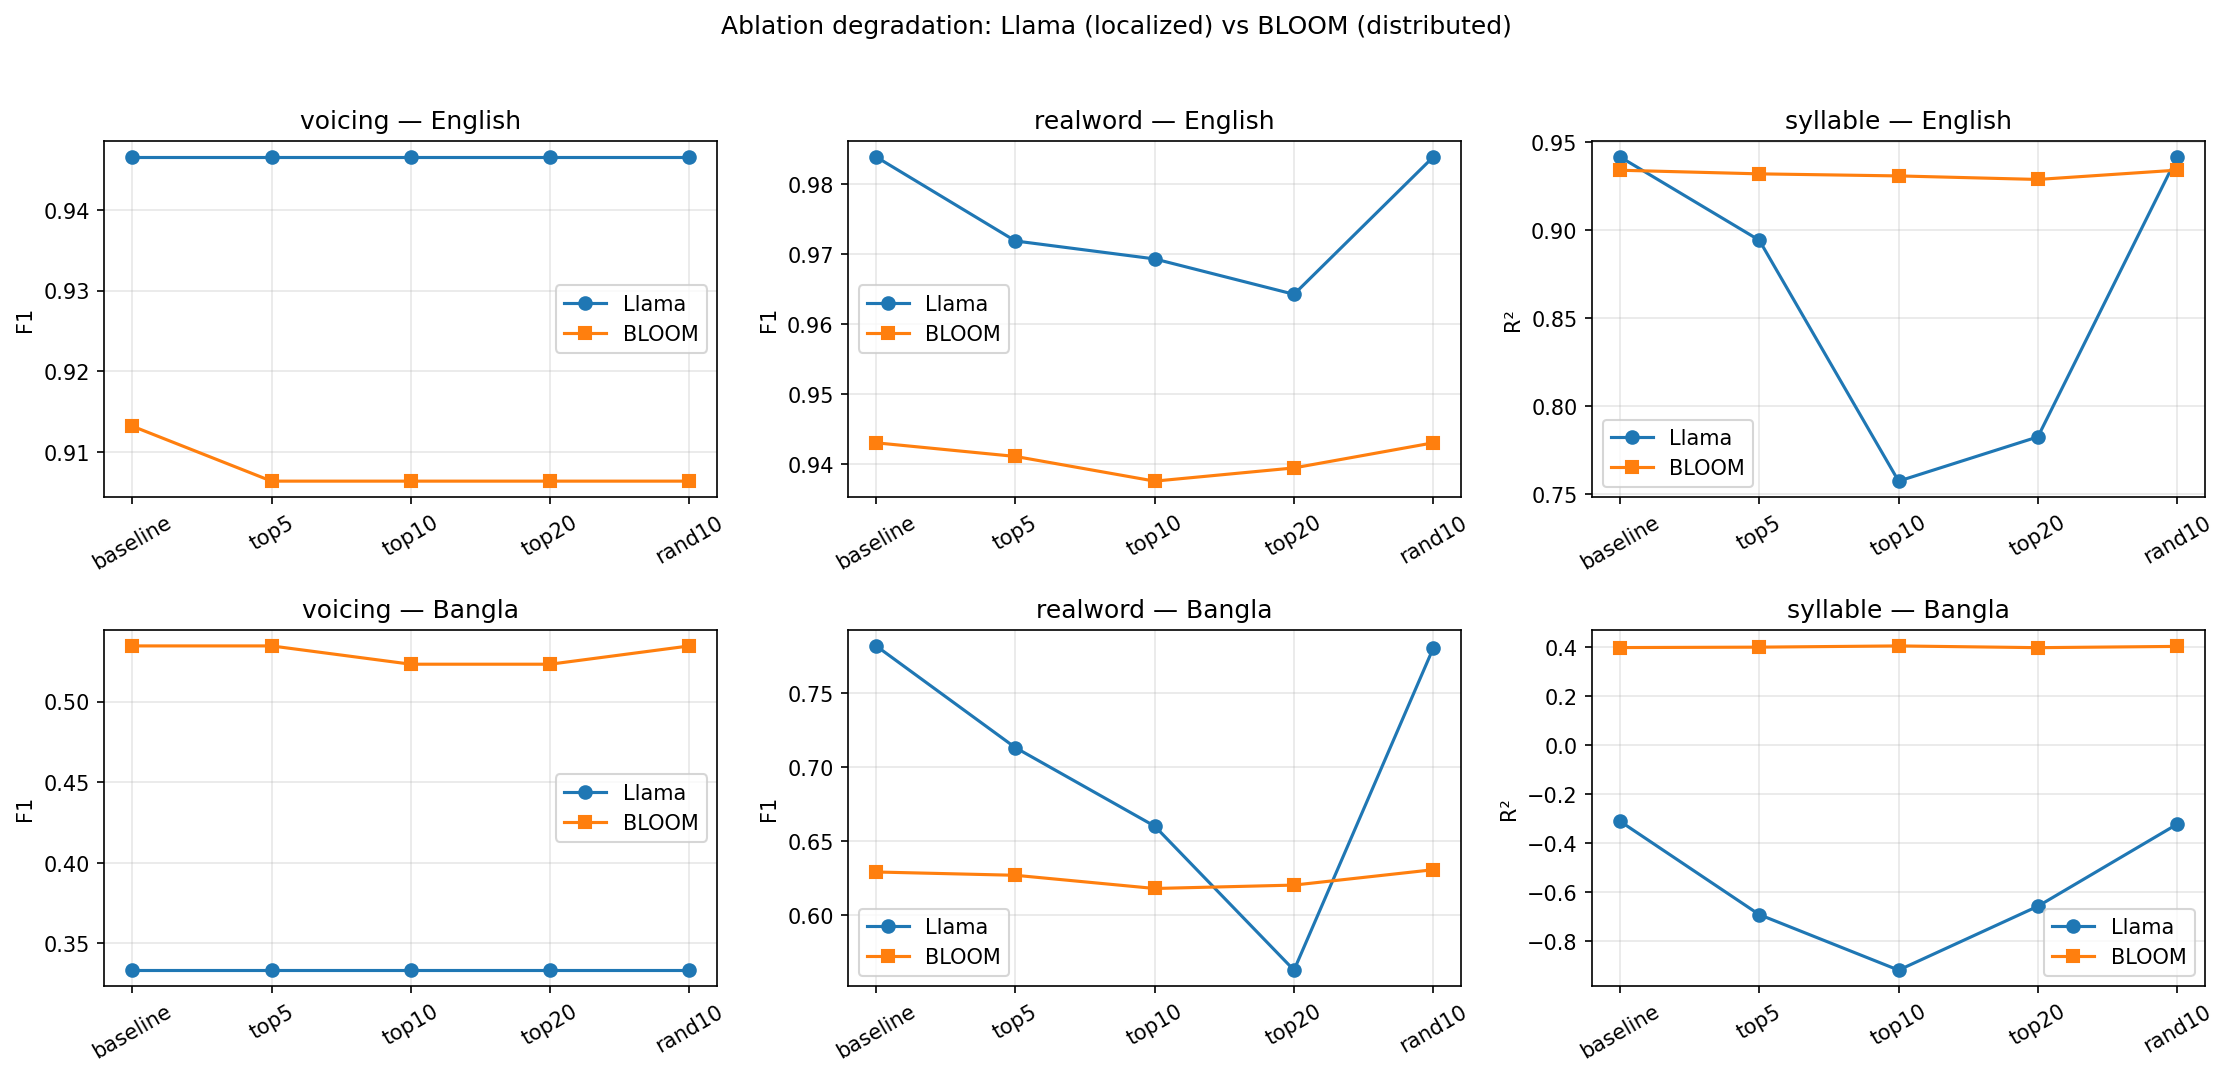
\includegraphics[width=0.85\textwidth]{plots_ablation_llama_vs_bloom.png}
\caption{Llama versus BLOOM ablation degradation curves on length-matched realword. The two decoder-only models diverge: BLOOM's distributed encoding tolerates top-20 ablation; Llama has no Bangla transfer to disrupt in the first place.}
\label{fig:llama-bloom}
\end{figure}

\begin{figure}[H]
\centering
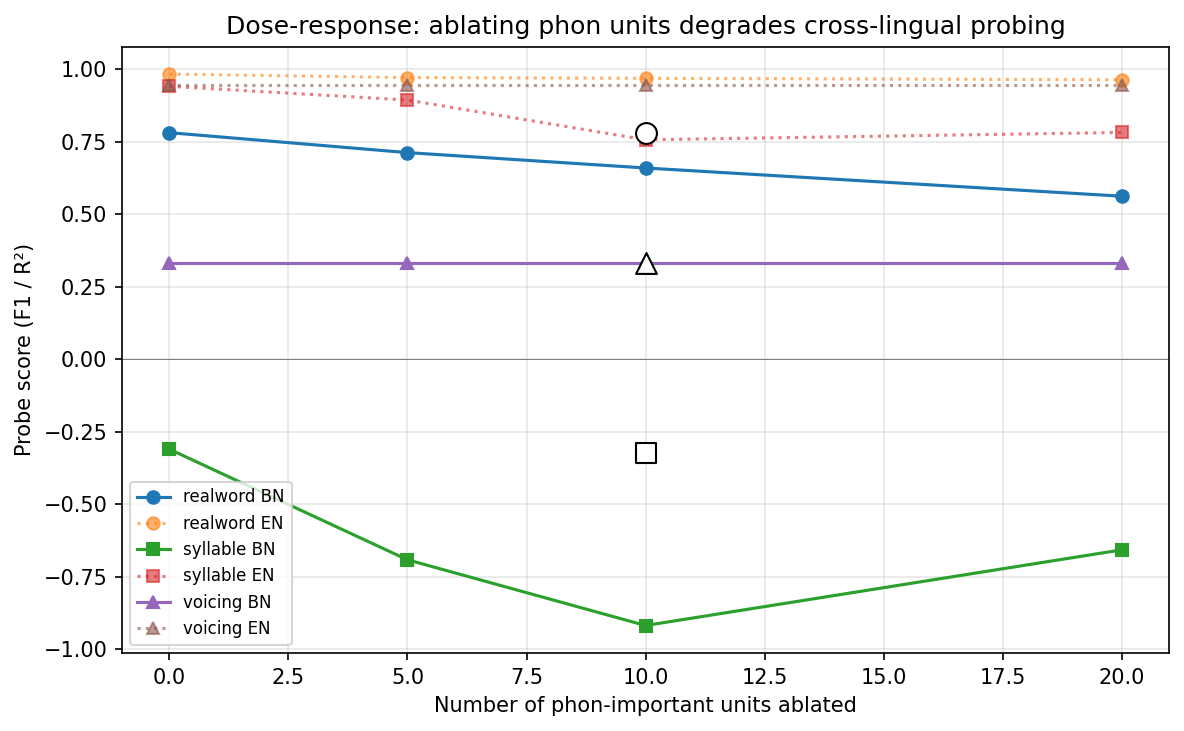
\includegraphics[width=0.85\textwidth]{plots_ablation_doseresponse_llama.png}
\caption{Llama dose-response ablation: BN F1 as a function of the number of zeroed top-ranked units. The curve sits at the chance line, confirming the absence of a localised cross-lingual lexical signal.}
\label{fig:doseresponse-llama}
\end{figure}

\subsection{mT5 localisation across encoder depth (RQ3 extension)}
\label{sec:mt5-localisation}

The L20 ablation showed a $+0.11$ specificity on mT5 (Table~\ref{tab:ablation-four}); a natural follow-up is whether this localisation is a property of the single \texttt{measure\_L} chosen or persists across the encoder. To answer this, the mT5 ablation is repeated at five depths (\texttt{measure\_L} $\in \{4, 8, 12, 16, 20\}$) with three random-unit-control seeds per depth, and the top-10 probe-ranked units at each depth are tracked by Jaccard overlap across depths.

\subsubsection{Localisation persists across encoder depth}

\begin{table}[H]
\centering
\caption{mT5 encoder ablation across depth. Top-10 versus random-mean specificity per measure\_L. Localisation persists across encoder depth; mid-encoder (L12) is strongest.}
\label{tab:mt5-depth}
\small
\resizebox{\textwidth}{!}{%
\setlength{\tabcolsep}{10pt}
\renewcommand{\arraystretch}{2}
\begin{tabular}{|c|c|c|c|c|}
\hline
\textbf{measure\_L} & \textbf{BN baseline} & \textbf{top10 drop} & \textbf{rand mean $\pm$ std} & \textbf{specificity} \\
\hline
L4   & 0.48 & $+0.06$ & $0.00 \pm 0.00$ & $+0.06$ \\
\hline
L8   & 0.49 & $+0.07$ & $0.00 \pm 0.00$ & $+0.07$ \\
\hline
\textbf{L12}  & \textbf{0.56} & $\bm{+0.14}$ & $0.01 \pm 0.01$ & $\bm{+0.13}$ \\
\hline
L16  & 0.56 & $+0.03$ & $-0.01 \pm 0.01$ & $+0.04$ \\
\hline
L20  & 0.60 & $+0.11$ & $0.00 \pm 0.00$ & $+0.11$ \\
\hline
\end{tabular}%
}
\end{table}

Specificity is positive at all five probed depths (range $+0.04$ to $+0.13$); random-unit drops are essentially zero across depths and seeds. mid-encoder L12 shows the strongest effect ($+0.13$), with L8 ($+0.07$) and L20 ($+0.11$) close behind. The result is not a single-layer fluke; it is an architectural property of the mT5 encoder.

\subsubsection{Two persistent backbone units, plus layer-local circuits}

The top-10 probe-ranked units per depth overlap modestly but non-trivially. Chance Jaccard overlap of two size-10 sets drawn from 2048 units is approximately $0.002$; observed pairwise overlaps reach $0.25$ between L4 and L8 and $0.18$ between L8/L12 and L12/L16 (Table~\ref{tab:mt5-overlap}), which is two orders of magnitude above chance.

\begin{table}[H]
\centering
\caption{Top-10 probe-ranked unit Jaccard overlap across mT5 encoder depths. Chance overlap is $\approx 0.002$.}
\label{tab:mt5-overlap}
\small
\resizebox{\textwidth}{!}{%
\setlength{\tabcolsep}{10pt}
\renewcommand{\arraystretch}{2}
\begin{tabular}{|c|c|c|c|c|c|}
\hline
 & \textbf{L4} & \textbf{L8} & \textbf{L12} & \textbf{L16} & \textbf{L20} \\
\hline
\textbf{L4}   & 1.00 & 0.25 & 0.05 & 0.11 & 0.00 \\
\hline
\textbf{L8}   & 0.25 & 1.00 & 0.18 & 0.18 & 0.05 \\
\hline
\textbf{L12}  & 0.05 & 0.18 & 1.00 & 0.18 & 0.05 \\
\hline
\textbf{L16}  & 0.11 & 0.18 & 0.18 & 1.00 & 0.05 \\
\hline
\textbf{L20}  & 0.00 & 0.05 & 0.05 & 0.05 & 1.00 \\
\hline
\end{tabular}%
}
\end{table}

Two units appear in the top-10 at four out of five probed depths: \textbf{u782} (in the top-10 at L4, L8, L12, L16) and \textbf{u1880} (in the top-10 at L8, L12, L16, L20). Of the 38 unique units that appear in any top-10 set across the five depths, 31 are layer-specific (appear at only one depth). The pattern is therefore \emph{hybrid}: a small persistent backbone of two cross-depth units, plus a much larger pool of layer-local specialised circuits, with graceful hand-off between them as depth increases. Neither a purely static channel theory (in which the same units carry the same information at every layer) nor a purely dynamic routing theory (in which each layer uses an entirely fresh set of units) fits the data; the truth is a mixture.

\begin{figure}[H]
\centering
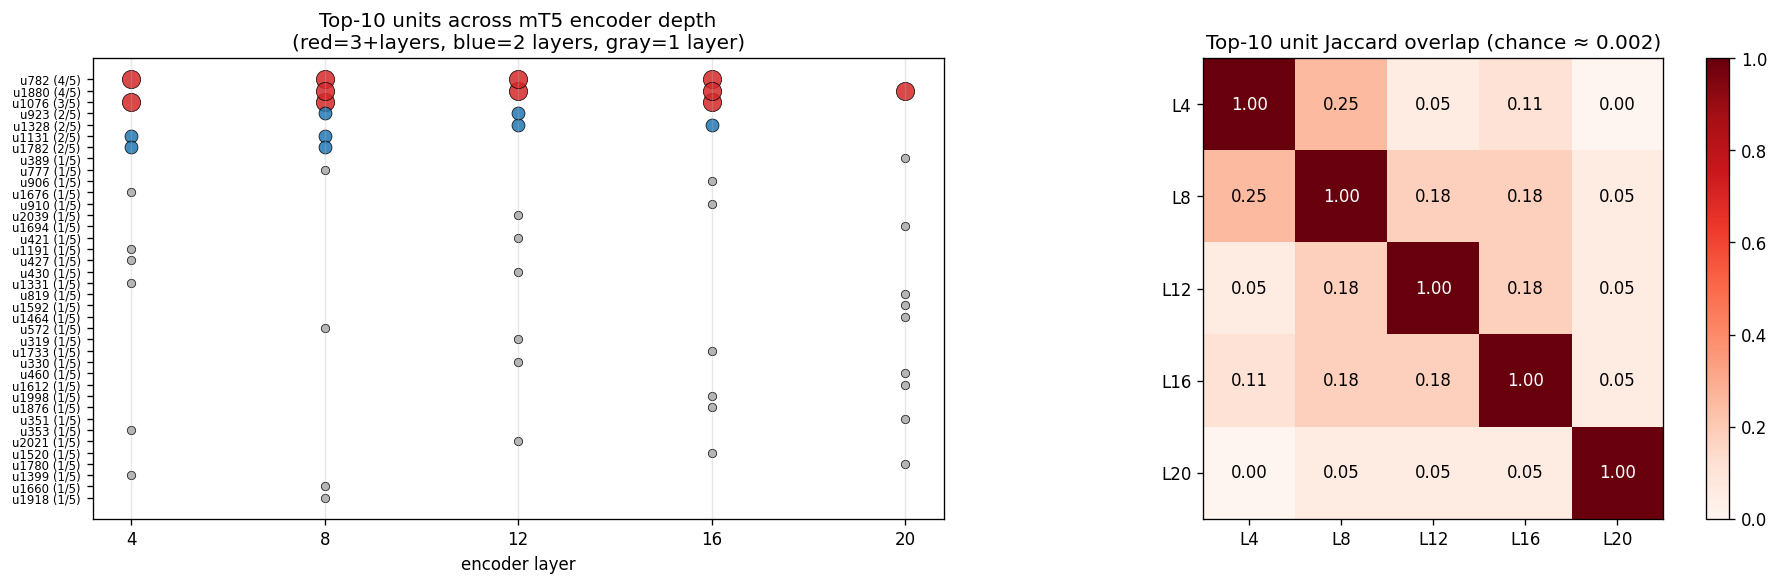
\includegraphics[width=0.85\textwidth]{plots_mt5_unit_overlap.png}
\caption{mT5 top-10 probe-ranked unit overlap (Jaccard) across encoder depths. Two persistent backbone units \{\textbf{u782}, \textbf{u1880}\} recur at $\geq 4$ of the 5 probed depths each; 31 of 38 unique top-10 units are layer-specific.}
\label{fig:mt5-overlap}
\end{figure}

\section{Final Design Adjustments}
\label{sec:adjustments}

Two design adjustments were made as a direct consequence of the results above.

First, the original RQ1 set of four phonological tasks (voicing, realword, ortho, syllable) was reduced to one (length-matched realword) for all RQ2 and RQ3 reporting, on the basis of Section~\ref{sec:sanity}. The original tables for the other three tasks are kept in Table~\ref{tab:rq1-en} only as the baseline against which the surface-feature failure is documented. This pruning is the central methodology contribution of the thesis.

Second, the ablation analysis was extended from a single \texttt{measure\_L} to a five-depth scan with three random-unit-control seeds per depth, after the L20 ablation showed a $+0.11$ specificity on mT5 (Table~\ref{tab:ablation-four}). The depth-scan result (Table~\ref{tab:mt5-depth}) and the Jaccard overlap analysis (Table~\ref{tab:mt5-overlap}, Figure~\ref{fig:mt5-overlap}) together establish the two-backbone-units finding (\{u782, u1880\}), which is the central mechanism contribution of the thesis.

\section{Statistical Analysis}
\label{sec:stats}

Probe performance is reported at the peak layer with the cross-validated mean across a 5-fold split of the English training set. Reported numbers are point estimates rather than confidence intervals because the length-matched subsets are small ($n = 50$ per language) and per-fold variance is dominated by stimulus-level idiosyncrasy. Where reported, ablation random-unit controls use three independent random seeds; the standard deviation across seeds is reported in Table~\ref{tab:mt5-depth} (typically $\leq 0.01$).

The persistence of u782 and u1880 across encoder depths is established by exhaustive enumeration of the top-10 probe-ranked units per depth, not by a statistical test. The relevant null is the chance Jaccard overlap of two random size-10 sets drawn from 2048 units, which is approximately $0.002$. The observed pairwise overlaps in Table~\ref{tab:mt5-overlap} range from $0.05$ to $0.25$ for the depth pairs that share at least one backbone unit; even the smallest of these observed values is roughly $25\times$ above chance, and the largest is roughly $125\times$ above chance. The backbone finding is therefore not a chance recurrence.

\section{Comparisons and Relationships}
\label{sec:comparisons}

\subsection{RQ4: Cross-model comparison and model selection}
\label{sec:rq4}

\subsubsection{Five comparative observations}

\begin{enumerate}
    \item \textbf{Best cross-lingual transfer (length-matched BN F1):} BLOOM ($0.92$, $+0.30$ over surface) $>$ XLM-R ($0.86$, $+0.24$) $\gg$ Llama ($0.63$, $+0.01$) $>$ mT5 ($0.60$, $-0.02$).
    \item \textbf{Best parameter efficiency:} XLM-R reaches $0.86$ BN F1 at $0.56$B parameters, roughly $13\times$ smaller than BLOOM ($7.1$B). Multilingual MLM-encoder pretraining is highly parameter-efficient for cross-lingual lexical structure.
    \item \textbf{Best in-language English realword:} Llama ($0.96$) $>$ BLOOM ($0.94$). English-causal pretraining dominates in English; the gap reverses cross-lingually.
    \item \textbf{Best causal localisation:} mT5 alone shows clean ablation specificity ($+0.11$ at L20, $+0.13$ at L12), with two persistent backbone units (u782, u1880) spanning the encoder. No other model in the comparison localises the cross-lingual lexical signal.
    \item \textbf{Pretraining objective and coverage dominate scale.} A $0.56$B multilingual encoder (XLM-R) beats an $8$B English-heavy decoder (Llama) on cross-lingual transfer; depth and width do not compensate for pretraining-language gaps.
\end{enumerate}

\subsubsection{Model-selection: paired recommendation}

The four models are not interchangeable; each dominates a different criterion. The thesis therefore issues a \emph{paired} recommendation rather than a single best-model claim:

\begin{itemize}
    \item \textbf{For a practical low-resource Bangla screening prototype:} BLOOM 7B1. Highest cross-lingual transfer ($0.92$ Bangla F1), survives surface controls, can be deployed as a frozen feature extractor without fine-tuning.
    \item \textbf{For interpretability and mechanism studies:} mT5 XL. The only model in the comparison whose cross-lingual lexical signal localises to a small unit set with a persistent two-unit backbone.
    \item \textbf{For hardware-constrained deployments:} XLM-RoBERTa large. At $0.56$B parameters it delivers $0.86$ Bangla F1 and runs in 16-bit on a single consumer GPU.
    \item \textbf{Not recommended:} Llama 3.1 8B for any cross-lingual Bangla setting at the lexical level. Length-matched transfer collapses to $0.63$ Bangla F1 (gain $+0.01$ over surface).
\end{itemize}

\subsection{Relationship to prior work}

The cross-lingual transfer numbers for XLM-R and BLOOM are consistent with the broader multilingual probing literature \cite{conneau2020xlmr,wu2020emerging,pires2019mbert}, but the gain-over-surface numbers we report are smaller than the gain-over-chance numbers commonly reported in earlier work. The difference is fully explained by the first-character lookup baseline and the length-matching control. The mT5 localisation result is new: prior interpretability work on multilingual models reports language-neutral and language-specific neurons in masked encoders \cite{stanczak2022neurons}, but not concentrated cross-lingual lexical coding with persistent backbone units in an encoder-decoder.

\section{Discussion}
\label{sec:discussion}

\subsection{Interpretation}

The headline finding is the joint role of pretraining objective and pretraining language coverage. The two transferring models (XLM-R and BLOOM) both have explicit Bangla coverage in their pretraining mix; the two collapsing models do not, in two different ways. Llama lacks Bangla coverage entirely; mT5 has multilingual coverage but its span-corruption objective does not surface cross-lingual lexical similarity at the probe-readable level on the length-matched task. BLOOM's multilingual causal-LM pretraining produces \emph{distributed} lexical representations that transfer well in raw performance but resist localisation; mT5's span-corruption encoder-decoder pretraining produces \emph{concentrated} lexical representations that survive at the unit level but do not surface in the length-matched cross-lingual probe at high F1. The two models are therefore complementary along the practical-vs-interpretable axis: BLOOM is the practical substrate, mT5 is the interpretability substrate.

The mT5 backbone-plus-routing pattern established in Section~\ref{sec:mt5-localisation} is itself a non-trivial mechanism finding. The hybrid organisation -- two persistent backbone units coexisting with a larger pool of layer-local circuits -- suggests a graceful hand-off architecture inside the mT5 encoder that, to our knowledge, has not been previously documented for multilingual lexical content.

\subsection{Implications}

For practitioners, the implications follow directly from the paired recommendation of Section~\ref{sec:rq4} and are not re-enumerated here: the substrate should be chosen against the deployment goal -- raw cross-lingual transfer, interpretability, or parameter efficiency -- because no single model dominates all three axes.

For the probing literature, the implication is methodological: the first-character lookup baseline (or its equivalent in the target language) and the length-matching control should be standard preconditions for any phonological probing claim. Three of four standard tasks in our setting fail these controls, and the cross-lingual signal reported in prior work likely reflects character statistics or token identity to a greater extent than usually acknowledged.

\subsection{Limitations}
\label{sec:caveats}

Five limitations bound the interpretation.

\begin{itemize}
    \item Bangla voicing labels in the original stimulus set are recoverable from the first character; the original \texttt{voiced\_unvoiced} column for Bangla is unusable for phonological probing as posed, and all Bangla voicing numbers in the original RQ1--RQ3 tables reflect first-character recognition.
    \item Length-matched subsets are small ($n = 50$ per language). Per-layer scores have meaningful variance; the gain-over-surface numbers are point estimates.
    \item The frozen probe English baseline reaches $1.00$ after matching; only the Bangla drop is interpretable as a causal signal in the ablation.
    \item Architectural confound: mT5 is the only encoder-decoder probed. The mT5 localisation result could reflect the span-corruption objective, the encoder-decoder split, or both; resolving this would require probing additional encoder-decoder models (e.g.\ ByT5, T5).
    \item BLOOM's ablation specificity is marginally negative ($-0.02$): zeroing the top-20 probe-ranked units \emph{slightly improves} Bangla transfer, which is consistent with distributed redundancy rather than a clean null. This is reported honestly rather than masked.
\end{itemize}